%%
% The BIThesis Template for Bachelor Graduation Thesis
%
% 北京理工大学毕业设计(论文)第一章节 —— 使用 XeLaTeX 编译
%
% Copyright 2020-2021 BITNP
%
% This work may be distributed and/or modified under the
% conditions of the LaTeX Project Public License, either version 1.3
% of this license or (at your option) any later version.
% The latest version of this license is in
%   http://www.latex-project.org/lppl.txt
% and version 1.3 or later is part of all distributions of LaTeX
% version 2005/12/01 or later.
%
% This work has the LPPL maintenance status `maintained'.
%
% The Current Maintainer of this work is Feng Kaiyu.
%
% 第二章

\chapter{理论基础及相关技术}

\section{代理内核操作系统实验}

\subsection{代理内核的概念}

代理内核(Proxy Kernel)是一种特殊的操作系统内核。
代理内核系统是由代理内核和Host主机的操作系统Ubuntu组成的。
代理内核与Host主机的操作系统之间使用HTIF接口进行通信。

代理内核并不是一个独立的操作系统,它虽然拥有I/O功能,但它不具备I/O的独立实现。
它的I/O功能实现依赖于Host主机的操作系统Ubuntu。
也就是说,代理内核Proxy Kernel与Host主机的操作系统Ubuntu是并行在运行的。
它们之间通过HTIF(Host Target Interface)通信。
当代理内核需要进行I/O时,代理内核就通过HTIF调用Host主机的操作系统Ubuntu的I/O接口,以达到I/O的目的。

\subsection{代理内核的思想}

代理内核是操作系统的最小集。
它只关心内存和CPU的管理,不关心外部设备I/O功能的实现。
代理内核的I/O功能都代理给Host主机的操作系统Ubuntu。
这样做的好处是,开发者不必在拘泥于繁琐的外部设备的I/O实现,
而是将注意力集中于计算机的核心资产CPU、内存等。

除此之外,因为代理内核少了具体的I/O实现,代理内核的代码会变得加更精简。
精简的代理内核代码更便于维护,也更便于后续学习者学习。

代理内核还有助于我们快速验证CPU软核。由于代理内核只关心CPU的管理,内存的管理。
这么一来,我们就可以将代理内核运行在更加独立的RISC-V CPU软核上,该CPU软核不需要实现I/O功能。
我们也可以更加集中精力去验证CPU软核的功能。从而进行快速的迭代和开发。
在真实的物理环境Zedboard开发板上,
代理内核的代码会被编译成RISC-V指令,
最终运行在FPGA上的RISC-V CPU软核上。
与此同时,Zedboard开发板上的ARM物理核运行着ARM版本的Ubuntu操作系统。
代理内核通过Zedboard上的HTIF接口调用Ubuntu的I/O接口,以达到I/O的目的。
这种设计下,我们不需要实现CPU的I/O功能,我们可以快速对RISC-V CPU软核进行验证。\cite{郭勇2019RISC}

\subsection{代理内核实验的基本介绍}

代理内核实验PKE主要分为三个部分:
a.系统调用、异常处理、时钟中断,b.内存管理,c.进程管理。
后面的实验对前面的实验具有依赖关系,如果前面的实验没有完成,后面的实验就不能进行。
每个实验都具有用户态程序、内核态程序。
实验操作者需要根据用户态程序的需求,补全内核代码。
只有这样,代理内核自身和用户程序才能正常运行。

代理内核实验PKE的每个小实验都较为精简紧凑。
对于实验操作者来说,在梳理好每个实验执行流程之后,就可以很容易对实验代码进行补全。
实验代码短小精悍,行数虽然少,但是代码的意义却很大。
它可以帮助实验操作者集中精力于管理计算机的内存、CPU,帮助实验操作者快速验证操作系统的理论知识。


\section{RISC-V新型开放指令集和精简指令集介绍}

\subsection{RISC-V的基本介绍}

RISC-V指令集是一种新型的开放和精简指令集。
它通过取长补短的方式,吸取了以往CPU指令集的优点、避免了以往CPU指令集的大部分缺点。

它是一个基于开放架构的指令集,RISC-V的指令是开放的,任何人都可以根据这个开放的指令集去实现RISC-V架构的CPU。
因此,RISC-V指令集具有开源、免费的特点。

它是一个精简的指令集。RISC-V手册指出,
同样的C语言程序,经过适用于不同CPU架构的编译器编译后,
得到的指令序列中,RISC-V架构的指令是相对来说数量较少、较精简的。
这对减少嵌入式设备功耗具有重要的意义。\cite{2014The}

\subsection{RISC-V的特权架构}

RISC-V的特权架构主要分为三种模式:
机器模式(Machine-mode)、
监管者模式(Supervisor-mode)、
用户模式(User-mode)。\cite{2015The}

M模式是拥有最高级权限的模式,M模式的硬件线程完全掌控着寄存器、内存、I/O的控制权。
M模式具备拦截和处理异常与中断的能力。除此之外,它还可以将异常与中断托管给S模式。

S模式的产生,主要是为了解决存储碎片化的问题。
S模式之下,我们可以开启分页机制,使用基于页面的虚拟内存。
这种模式的特权级相比M模式较低。与M模式相比,S模式拥有的权限较少。
与U模式相比,S模式拥有的权限较多。
我们的操作系统内核PKE,主要就是运行在S模式。

U模式也就是用户态程序运行时的模式。
它具备最低的特权级,拥有的权限最少。
它所需的许多功能,都需要通过系统调用、中断、异常等机制获取。
它通过这些机制,让CPU的执行切换到更高特权级的内核中,
让内核来提供并执行用户态程序所需功能(如串口输出、定时器、异常处理等)。

这三种模式之间不是普通的链式关系,而是一层叠一层的金字塔结构。
更高特权级的底层为上层提供运行时服务,更低特权级的上层运行并依赖于底层之上。

\subsection{RISC-V的中断、异常委托}

前面我们提到,M模式具备拦截和处理异常与中断的能力。
M模式下运行的内核可以根据中断/异常的状态码和向量表选择对应的处理程序。
拦截和处理中断、异常。

除此之外,M模式还可以将这两者的拦截和处理委托给S模式的内核。
M模式的内核可以在初始化时,
通过设置异常委托寄存器(medeleg)、中断委托寄存器(mideleg),
将异常和中断的拦截与处理委托给S层。
M层的内核只需要在初始化时,根据异常、中断的状态码值,
在委托寄存器的对应二进制位赋值即可。
委托寄存器的初始化结束以后,寄存器上对应的异常/中断的拦截与处理都会交接给S模式的内核。

\section{现有内核在K210移植工作的参考}

\subsection{K210的基本信息}

\begin{figure}[htbp]
    \vspace{13pt} % 调整图片与上文的垂直距离
    \centering
    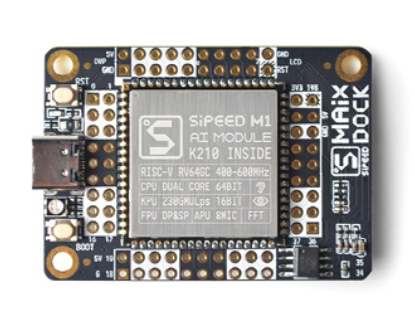
\includegraphics[width=0.6\textwidth]{images/K210.png}
    \caption{K210 MCU}\label{K210 MCU} % label 用来在文中索引
\end{figure}

K210是由嘉楠公司推出的一款MCU,它具有成本低、高性能、性价比高等特点。\cite{2018嘉楠科技勘智}

K210拥有基于RISC-V架构、64位的双核CPU。它具有6MB物理内存,它的晶振频率是400-600MHZ。
除此之外,它拥有嘉楠自研的神经网络计算加速器KPU,可以进行高性能的神经网络计算。

K210的成本低廉。一块不带其他外设的K210 MCU,只需要一百多元。
这样成本低廉的物理开发板对嵌入式开发、操作系统实验教学、学生自学计算机知识很有好处。

\subsection{THU ucore在K210的移植}

ucore是清华大学基于MIT开源的xv6内核开发的操作系统内核,
它可以运行在X86计算机上,也可以运行在X86硬件模拟器上,如QEMU、VirtualBox等。
麻雀虽小,五脏俱全。ucore的代码量不到5000行,
却包含了虚拟内存管理、进程管理、文件系统等主要内核功能。

早在2020年,南开大学的操作系统团队发起了ucore在RISC-V指令集CPU的移植活动。
从2020年3月到2020年4月,历时4个月,他们完成了ucore从X86物理机到RISC-V物理机的移植,
最终让ucore成功运行在RISC-V架构的K210上。

我们可以参考南开操作系统团队的\href{https://github.com/NKU-EmbeddedSystem/riscv64-ucore}{移植工作},来完成PKE的移植与改进。

\subsection{MIT xv6在K210的移植}

MIT的Frans Kaashoek等在2006年参考PDP-11上的UNIX Version 6写了一个可在X86上跑的操作系统xv6(基于MIT License)\cite{张治国2020Xv6}

华科的操作系统团队完成了xv6从X86物理机到RISC-V物理机的移植,
最终让xv6成功运行在K210上。

同理,我们可以参考华科操作系统团队的\href{https://github.com/HUST-OS/xv6-k210}{移植工作},来完成PKE的移植与改进。